\section{BPX Type: Model ('M')}

\subsection{Overview}
The Model BPX is using 'M' as the type byte of BPX Main Header. This type provides optimized and efficient mesh storage for 3D rendering APIs.
\newline
Below is a table describing the different sections to be expected in a BPXM:
\begin{center}
    {
        \rowcolors{2}
        {red!15}
        {blue!15}
        \begin{tabular}{|c|c|c|c|}
            \hline
            \textbf{Name} & \textbf{Type} & \textbf{Required} & \textbf{Single Time} \\
    
            \hline\hline
            VertexFormat & 0 & Yes & Yes \\
            VertexArray & 1 & Yes & No \\
            BoneArray & 2 & No & Yes \\
            FrameArray & 3 & No & Yes \\
            AnimationArray & 4 & No & Yes \\
            Strings & 5 & No & Yes \\
            \hline
        \end{tabular}
    }
\end{center}

\subsection{VertexFormat}
Contains information about the vertex format when attempting to present the model ro a rendering API.\newline
It is divided into two parts:
\begin{itemize}
    \item A header
    \item An array of data structures describing each vertex component
\end{itemize}
The header data structure is given by the following table:
\begin{center}
    {
        \rowcolors{2}
        {red!15}
        {blue!15}
        \begin{tabular}{|c|c|c|c|}
            \hline
            \textbf{Name} & \textbf{Type} & \textbf{Size} & \textbf{Notes} \\
    
            \hline\hline
            VertexSize & Unsigned & 16 & Total size in bytes of a single vertex \\
            NumComponents & Unsigned & 8 & Number of components \\
            Reserved & Unspecified & 8 & Blank, always 0 \\
            \hline
        \end{tabular}
    }
\end{center}
Each vertex component is represented using the following data structure:
\begin{center}
    {
        \rowcolors{2}
        {red!15}
        {blue!15}
        \begin{tabular}{|c|c|c|c|}
            \hline
            \textbf{Name} & \textbf{Type} & \textbf{Size} & \textbf{Notes} \\
    
            \hline\hline
            Type & Unsigned & 4 & Type of component \\
            Size & Unsigned & 4 & Size of component \\
            \hline
        \end{tabular}
    }
\end{center}

\subsubsection{VertexSize}
The size of a single vertex structure is determined by the summation of each individual component size in bytes, the formula is given by:
\begin{equation}
    S = \sum_{i=1}^{N} C_i \times D_i
\end{equation}
where $S$ is the size of a single vertex, $N$ is the number of components, $C_i$ is the size of the ith component and $D_i$ is the data type size of the ith component

\subsubsection{NumComponents}
The number of components that is expected to be read from the vertex component array.

\subsubsection{Type}
The data type for a given vertex component. Supported data types are:
\begin{center}
    {
        \rowcolors{2}
        {red!15}
        {blue!15}
        \begin{tabular}{|c|c|c|c|}
            \hline
            \textbf{Name} & \textbf{Value} & \textbf{Notes} \\

            \hline\hline
            FLOAT & 0x1 & A float component; 32 bits \\
            INT & 0x2 & A signed integer component; 32 bits \\
            UINT & 0x3 & An unsigned integer component; 32 bits \\
            \hline
        \end{tabular}
    }
\end{center}

\subsubsection{Size}
The component size; how many of data types should this vertex component have. As an example a Vector 3 of float would be represented as a data type FLOAT with a component size of 3.

\subsection{VertexArray}
This section contains a header followed by an array of vertex data structure. The size of each vertex structure should be equal to the field VertexSize in the VertexFormat section.\newline
The header data structure is described in the following table:
\begin{center}
    {
        \rowcolors{2}
        {red!15}
        {blue!15}
        \begin{tabular}{|c|c|c|c|}
            \hline
            \textbf{Name} & \textbf{Type} & \textbf{Size} & \textbf{Notes} \\
    
            \hline\hline
            Material & Unsigned & 32 & Pointer in the Strings section \\
            VertexCount & Unsigned & 32 & Total number of vertices \\
            \hline
        \end{tabular}
    }
\end{center}

\subsubsection{Material}
This field is a pointer to a null terminated string in the Strings section that is used to identify the Engine asset path of the default material to apply when rendering this vertex array.

\subsubsection{VertexCount}
The amount of vertex structures to read after this header.\newline
\textbf{We remind that all modern hardware support triangles as primitives, so the vertex count should be a multiple of 3}

\subsubsection{Total array size}
The total size in bytes of the vertex array to use as pre-allocation buffer size when loading this model can be calculated as follows:
\begin{equation}
    SA = S \times V
\end{equation}
where $SA$ is the total size of the vertex array, $S$ the size of a single vertex structure as given in the VertexFormat section and $V$ the number of vertices in the array given by the VertexCount field.\newline
To avoid storing an additional 64 bits field in the header of the VertexArray section this size $SA$ is left to be calculated by the implementing application.

\subsection{BoneArray}
This section contains a header followed by an array of data structures representing each bone in a skeletal mesh.\newline
Below is a description of the header to find before bone data in this section:
\begin{center}
    {
        \rowcolors{2}
        {red!15}
        {blue!15}
        \begin{tabular}{|c|c|c|c|}
            \hline
            \textbf{Name} & \textbf{Type} & \textbf{Size} & \textbf{Notes} \\
    
            \hline\hline
            BoneCount & Unsigned & 16 & Total number of bones \\
            \hline
        \end{tabular}
    }
\end{center}

Each bone in the array following the header is represented by the following data structure:
\begin{center}
    {
        \rowcolors{2}
        {red!15}
        {blue!15}
        \begin{tabular}{|c|c|c|c|}
            \hline
            \textbf{Name} & \textbf{Type} & \textbf{Size} & \textbf{Notes} \\
    
            \hline\hline
            InitTransform & float & 512 & Initial transform matrix \\
            Name & Unsigned & 32 & Pointer in the Strings section \\
            \hline
        \end{tabular}
    }
\end{center}

\subsubsection{BoneCount}
Number of bones to expect in the bone array following the header. This number should not be greater than 65535.

\subsection{Analysis on theoretical bone limit}
We can give an estimation that human skeleton can be up to 400 bones. Of course most models do not include as many bones to reduce GPU/CPU load.
\begin{itemize}
    \item OpenGL, Vulkan and Metal maximum UBO/function constants storage size available to a shader is usualy 64Kb or 65536 bytes
    \item On the official MSDN page \cite{MSDNConstantBuffers} for DirectX the maximum constant buffer size available to a shader is $4096 constants \times 432 bits = 4096 constants \times 54 bytes = 221184 bytes$
\end{itemize}
UBO, function constants and constant buffer refers to means of variable synchronisation between CPU accessible memory and GPU accessible memory. Vulkan is a special case as it actually supports faster memory called Push Constants, however these constants usually maxes at 256-512 bytes which is impracticable for storing bone transforms. Push constants are typically used to exchange important transformation matrices such as model, view or projection.
The size of a transformation matrix in 3D space using homogeneous coordinate system \cite{HomogeneousCoordinates} is $32 bits (float) \times 4 \times 4 (4\times4 matrix) = 16 \times 32 bits = 512 bits = 64 bytes$.\newline
So assuming the lowest size for storing bones in VRAM for GPU processing is $65536$ we can theoretically store up to $1024$ matrices assuming each bone matrix represents 3D space transformations in homogeneous coordinate system ($\frac{65536}{64} = 1024$).\newline
Which means in order to \textbf{keep compatibility} with as many platforms/rendering apis as possible also taking into account byte indexing, we should store the bone count as a 16 bits integer.

\subsubsection{InitTransform}
Initial transform matrix to apply to that specific bone, the matrix is expected to be in homogeneous coordinate system respecting the convention specified in the begining of this document.

\subsubsection{Name}
Bone name as a pointer to a null terminated string in the strings section.

\subsection{FrameArray}
This section contains a header followed by an array of data structures each representing the new transform for a combination of a bone and frame.\newline
The array should be organized as the following diagram describes:
\begin{figure}[h!]
    \centering
    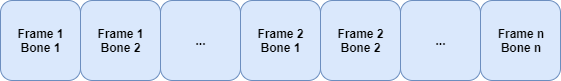
\includegraphics[scale=0.7]{Types/FrameArray_Diagram.png}
    \label{fig:FrameArray_Diagram}
    \caption{Diagram for organizing frame array}
\end{figure}

\subsubsection{Design decision}
The majority of mainstream formats represents animated models using key frames, that is storing only determinant changes in the model and interpolating intermediate frames at runtime. In BPX type M each frame is stored in the file to allow for any interpolation method, that is the interpolation if there's any is defined by the exporter of that model. The engine runtime does not have to provide any interpolation function for BPX type M.\newline
This change grants the \textbf{flexibility} of using any interpolation functions even user defined.